\documentclass{beamer}
\usepackage[english]{babel}
\usepackage{color} 
\usepackage{graphicx}
\usepackage{algorithm}
\usepackage{algorithmic}
%\usepackage{biblatex}
\usetheme{Warsaw}  

\setbeamertemplate{footline}[frame number]

\title[Fast brain decoding]{Fast brain decoding with random sampling and random 
projections}
\author{\textbf{Andr\'es HOYOS-IDROBO}, Ga\"el VAROQUAUX and Bertrand THIRION}
\institute{
\includegraphics[width=0.31\linewidth]{figures/parietal_logo.png}\quad
\includegraphics[width=0.21\linewidth]{figures/inria_logo.jpg}\quad

\includegraphics[width=0.21\linewidth]{figures/msr_logo.png}\quad

\includegraphics[width=0.11\linewidth]{figures/cea_logo.png}
}
\date{\textbf{PRNI 2016} - 6TH International Workshop on Pattern Recognition in 
Neuroimaging}


\begin{document}
\maketitle


\begin{frame}\frametitle{\textbf{Context:} Brain decoding}

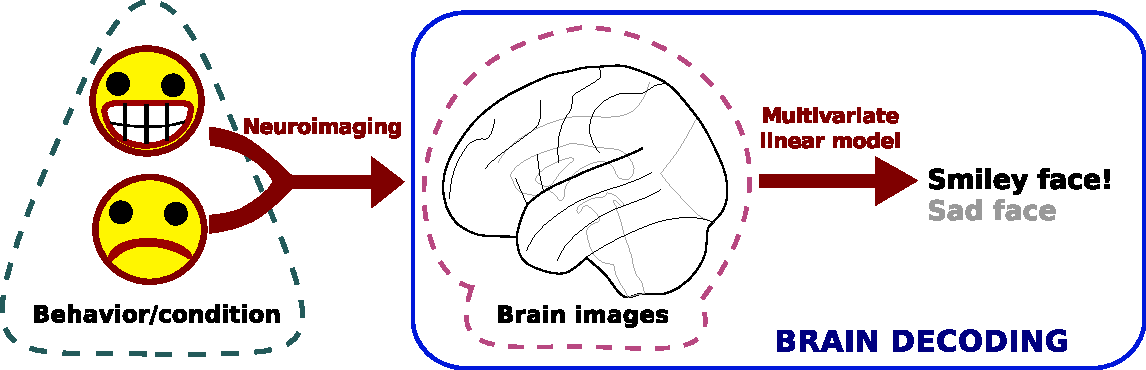
\includegraphics[width=1\linewidth]{figures/brain_decoding.pdf}

\begin{itemize}
\item \textbf{The goal:} To  link brain regions with experimental 
conditions/behaviors.
\item \textbf{We work with} a data matrix $\mathbf{X} \in \mathbb{R}^{n\times 
p}$, composed by $n$ images and $p$ voxels, where $p > n$.
\item \textbf{We use} linear methods $\rightarrow$ interpretability.
\end{itemize}

\begin{block}{}
\begin{itemize}
\item\textbf{We are interested on} large scale brain decoding problems. 
\item\textbf{We want} to \structure{\textbf{speedup}} linear classifiers on 
large datasets.
\end{itemize}
\end{block}

\end{frame}


\begin{frame}\frametitle{\textbf{Fast dimensionality reduction}}

We rely on \textbf{kernel-based methods}: 

\quad Feature transformation + linear method 

\begin{figure}
\centering
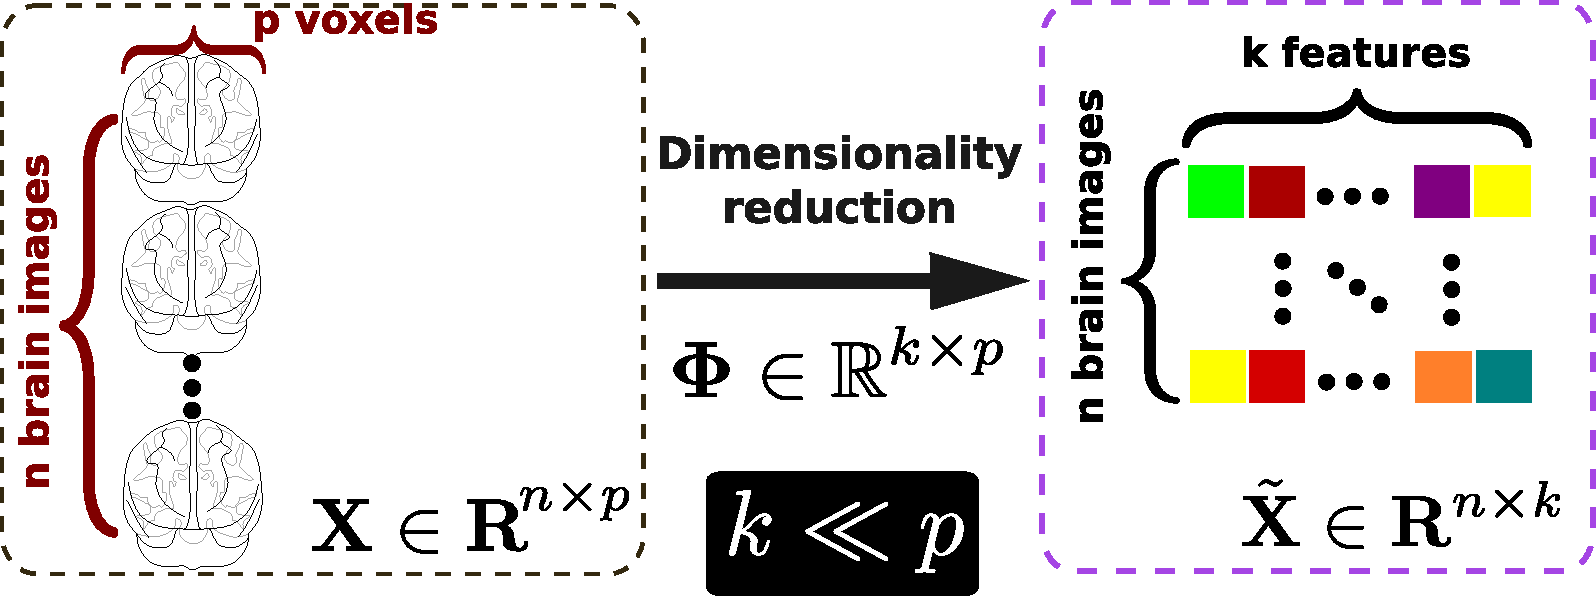
\includegraphics[width=1\linewidth]{figures/dim_reduction.pdf}
\end{figure}
\end{frame}


\begin{frame}\frametitle{\textbf{Matrix approximation:} By randomized methods}

\begin{itemize}
\item \textbf{Approximation by dimension reduction:} Randomly combine matrix 
columns (random projections).
\item \textbf{Random sampling:} Nystr\"om method (interpolative decomposition)
\end{itemize}
\end{frame}


\begin{frame}
\frametitle{\textbf{Dimension reduction by random projections}}

\begin{figure}
\centering
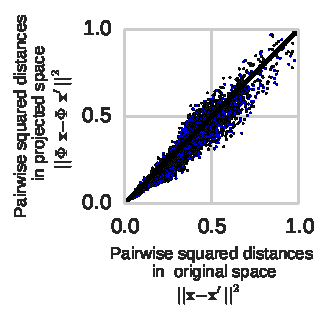
\includegraphics[width=0.4\linewidth]{figures/pairwise_distace.pdf}
\caption{Random projections preserve the pairwise squared distance in the 
projected 
space with a distortion up to $\epsilon$, where $k = O(\log(n)/\epsilon^2).$ }
\end{figure}

\begin{itemize}
\item Theoretical guaranties: approximation of pairwise 
distances.
\item It is data-agnostic.
\item It is difficult to bring to the brain space.
\end{itemize}
\end{frame}


\begin{frame}

\frametitle{\textbf{Random sampling:} Interpolative decomposition}
\begin{figure}
\centering
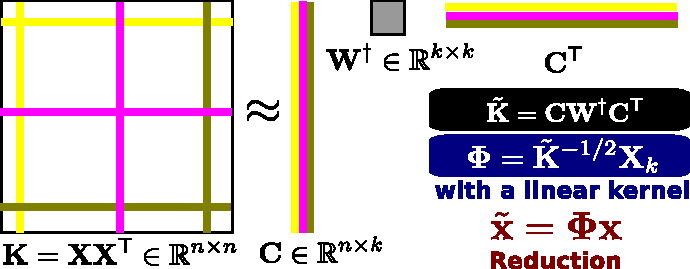
\includegraphics[width=0.75\linewidth]{figures/nystroem.pdf}
\end{figure}

Approximation by random sampling: randomly selecting a subset of rows
\begin{itemize}
    \item Mainly used to approximate a Gram matrix, $\mathbf{K} = 
    \mathbf{X}\,\mathbf{X}^\mathsf{T} \in \mathbb{R}^{n\times n}$.
    \item It is data-aware.
\end{itemize}
\end{frame}

\begin{frame}
\begin{algorithm}[H]
\caption{Nystr\"om method: Learning the feature mapping}
\begin{algorithmic}[1]
\REQUIRE The training data matrix $\mathbf{X} \in \mathbb{R}^{n\times p}$, 
number $k$ of 
components, where $k < n$.
\ENSURE The feature mapping $\mathbf{\Phi} \in \mathbb{R}^{k\times p}$ 
\STATE $\mathbf{r} \leftarrow$ Generate uniform sampling of $k$ components\\
\STATE $\mathbf{X}_{\mathbf{r}} \in \mathbb{R}^{k\times p}$ \COMMENT{Subsample 
of $k$ rows}\\
\STATE $\mathbf{K}_{\mathbf{r}} = \mathbf{X}_\mathbf{r} 
\mathbf{X}_\mathbf{r}^\mathsf{T}$ \COMMENT{Kernel 
matrix of the subsampled data}\\
\STATE $\mathbf{\Phi} = \mathbf{K}_\mathbf{r}^{-1/2} \mathbf{X}_\mathbf{r}$ 
\COMMENT{Normalization}\\
\RETURN $\mathbf{\Phi}$
\end{algorithmic}
\end{algorithm}

\end{frame}


\begin{frame}\frametitle{\textbf{Experimental setup:} Validating the 
approximation}

\begin{block}{}
\textbf{Goal:} Investigate decoding after random projections and random 
sampling. 

\textbf{Datasets:} Functional and anatomical brain images.

\begin{itemize}
\item Haxby: fMRI, visual object recognition.
\item OASIS: Voxel-based morphometry, gender discrimination.
\item Human Connectome Project (HCP): fMRI, 17 cognitive tasks. 
\end{itemize}

In all datasets $n > 180$
\end{block}
\end{frame}


\begin{frame}\frametitle{Benchmarking of linear classifiers}
\begin{figure}
\centering
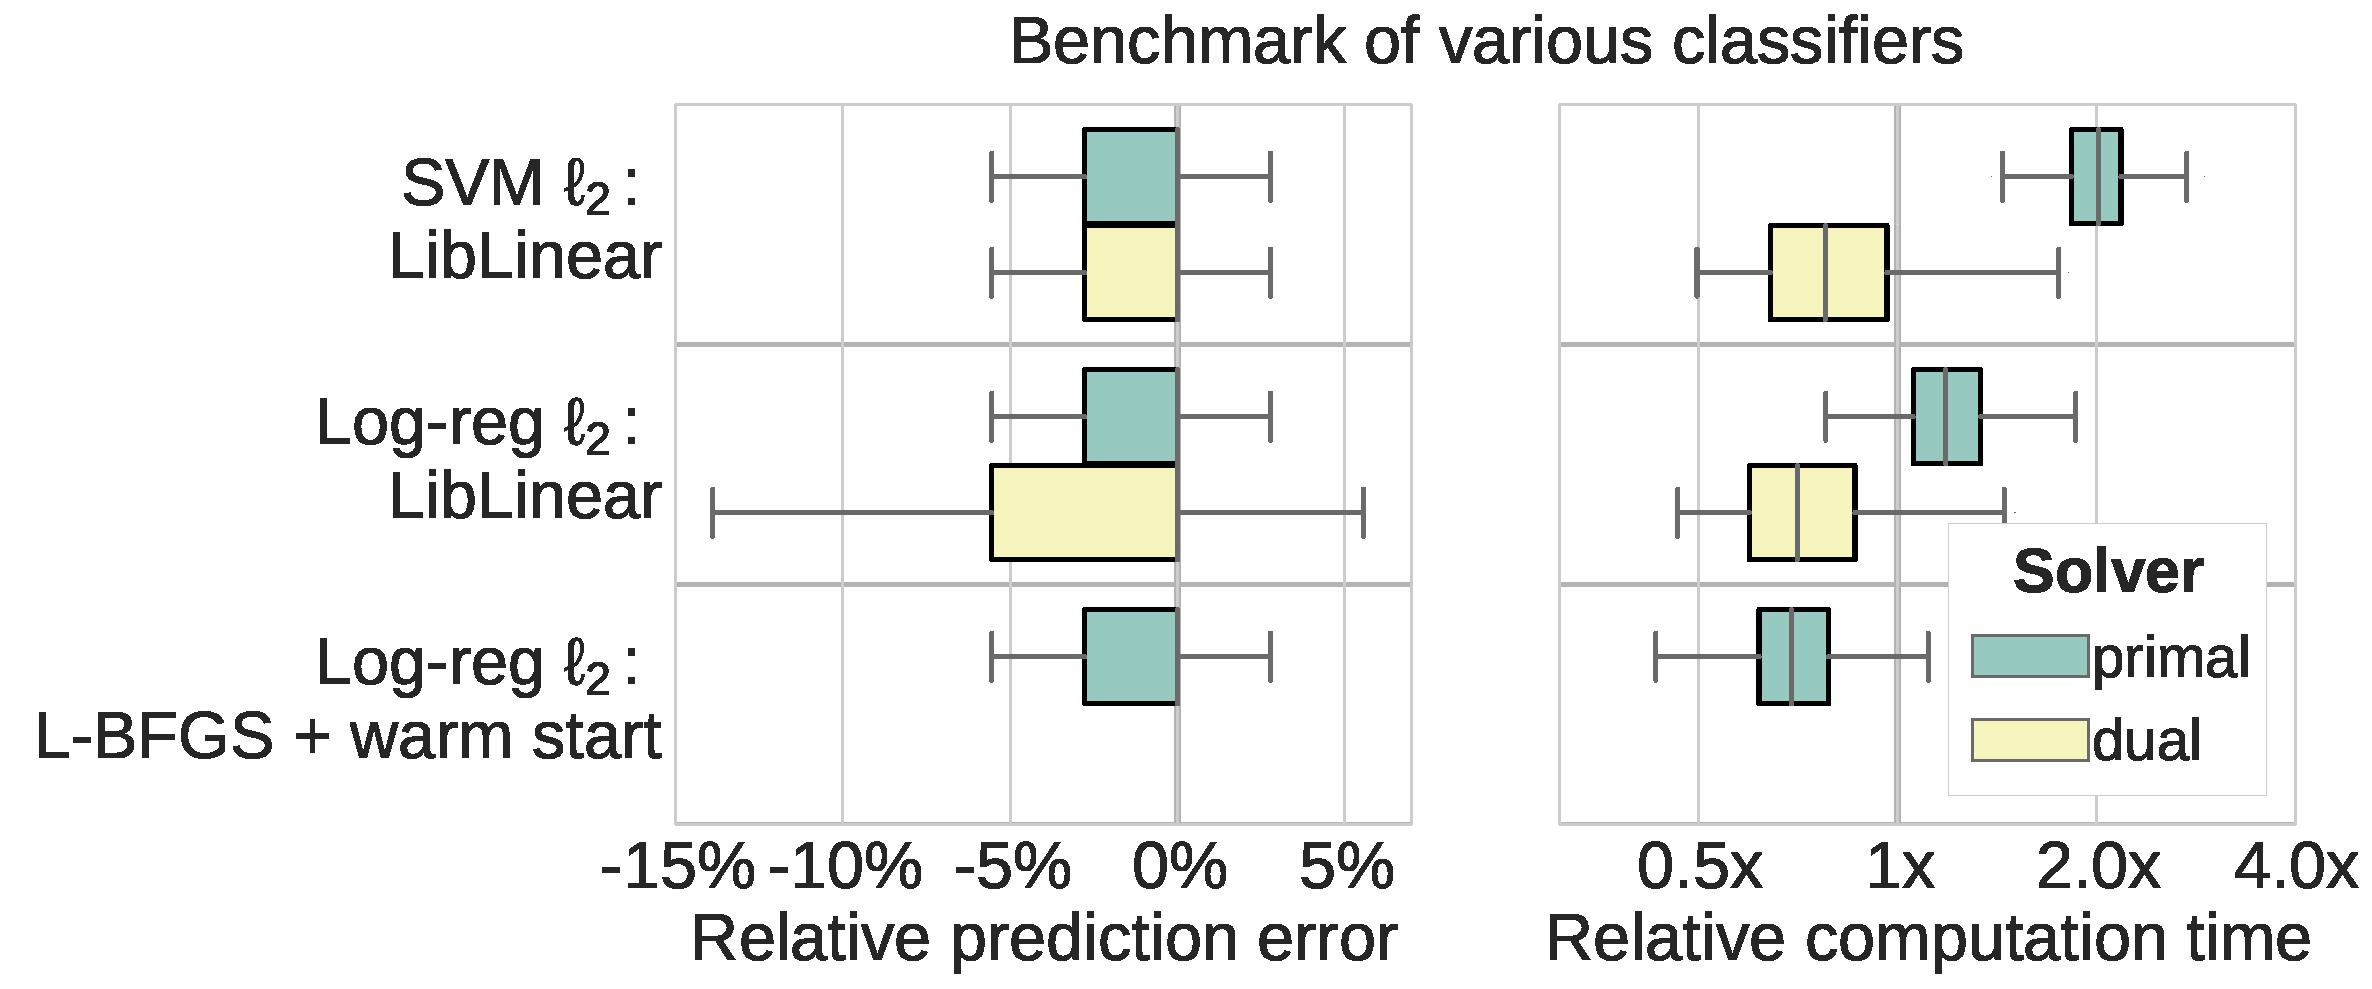
\includegraphics[width=1\linewidth]{figures/benchmark.pdf}
\caption{\textbf{Relative performance to LibSVM.} The logistic regression using 
L-BFGS with warm start, displays a good trade-off between computation time and 
accuracy.}
\end{figure}
\end{frame}


\begin{frame}\frametitle{Random sampling, Random projections and decoding}
\includegraphics[width=1\linewidth]{figures/comparison.pdf}
\end{frame}


\begin{frame}\frametitle{\textbf{Bringing the reduction to the brain space}}
\begin{figure}
\centering
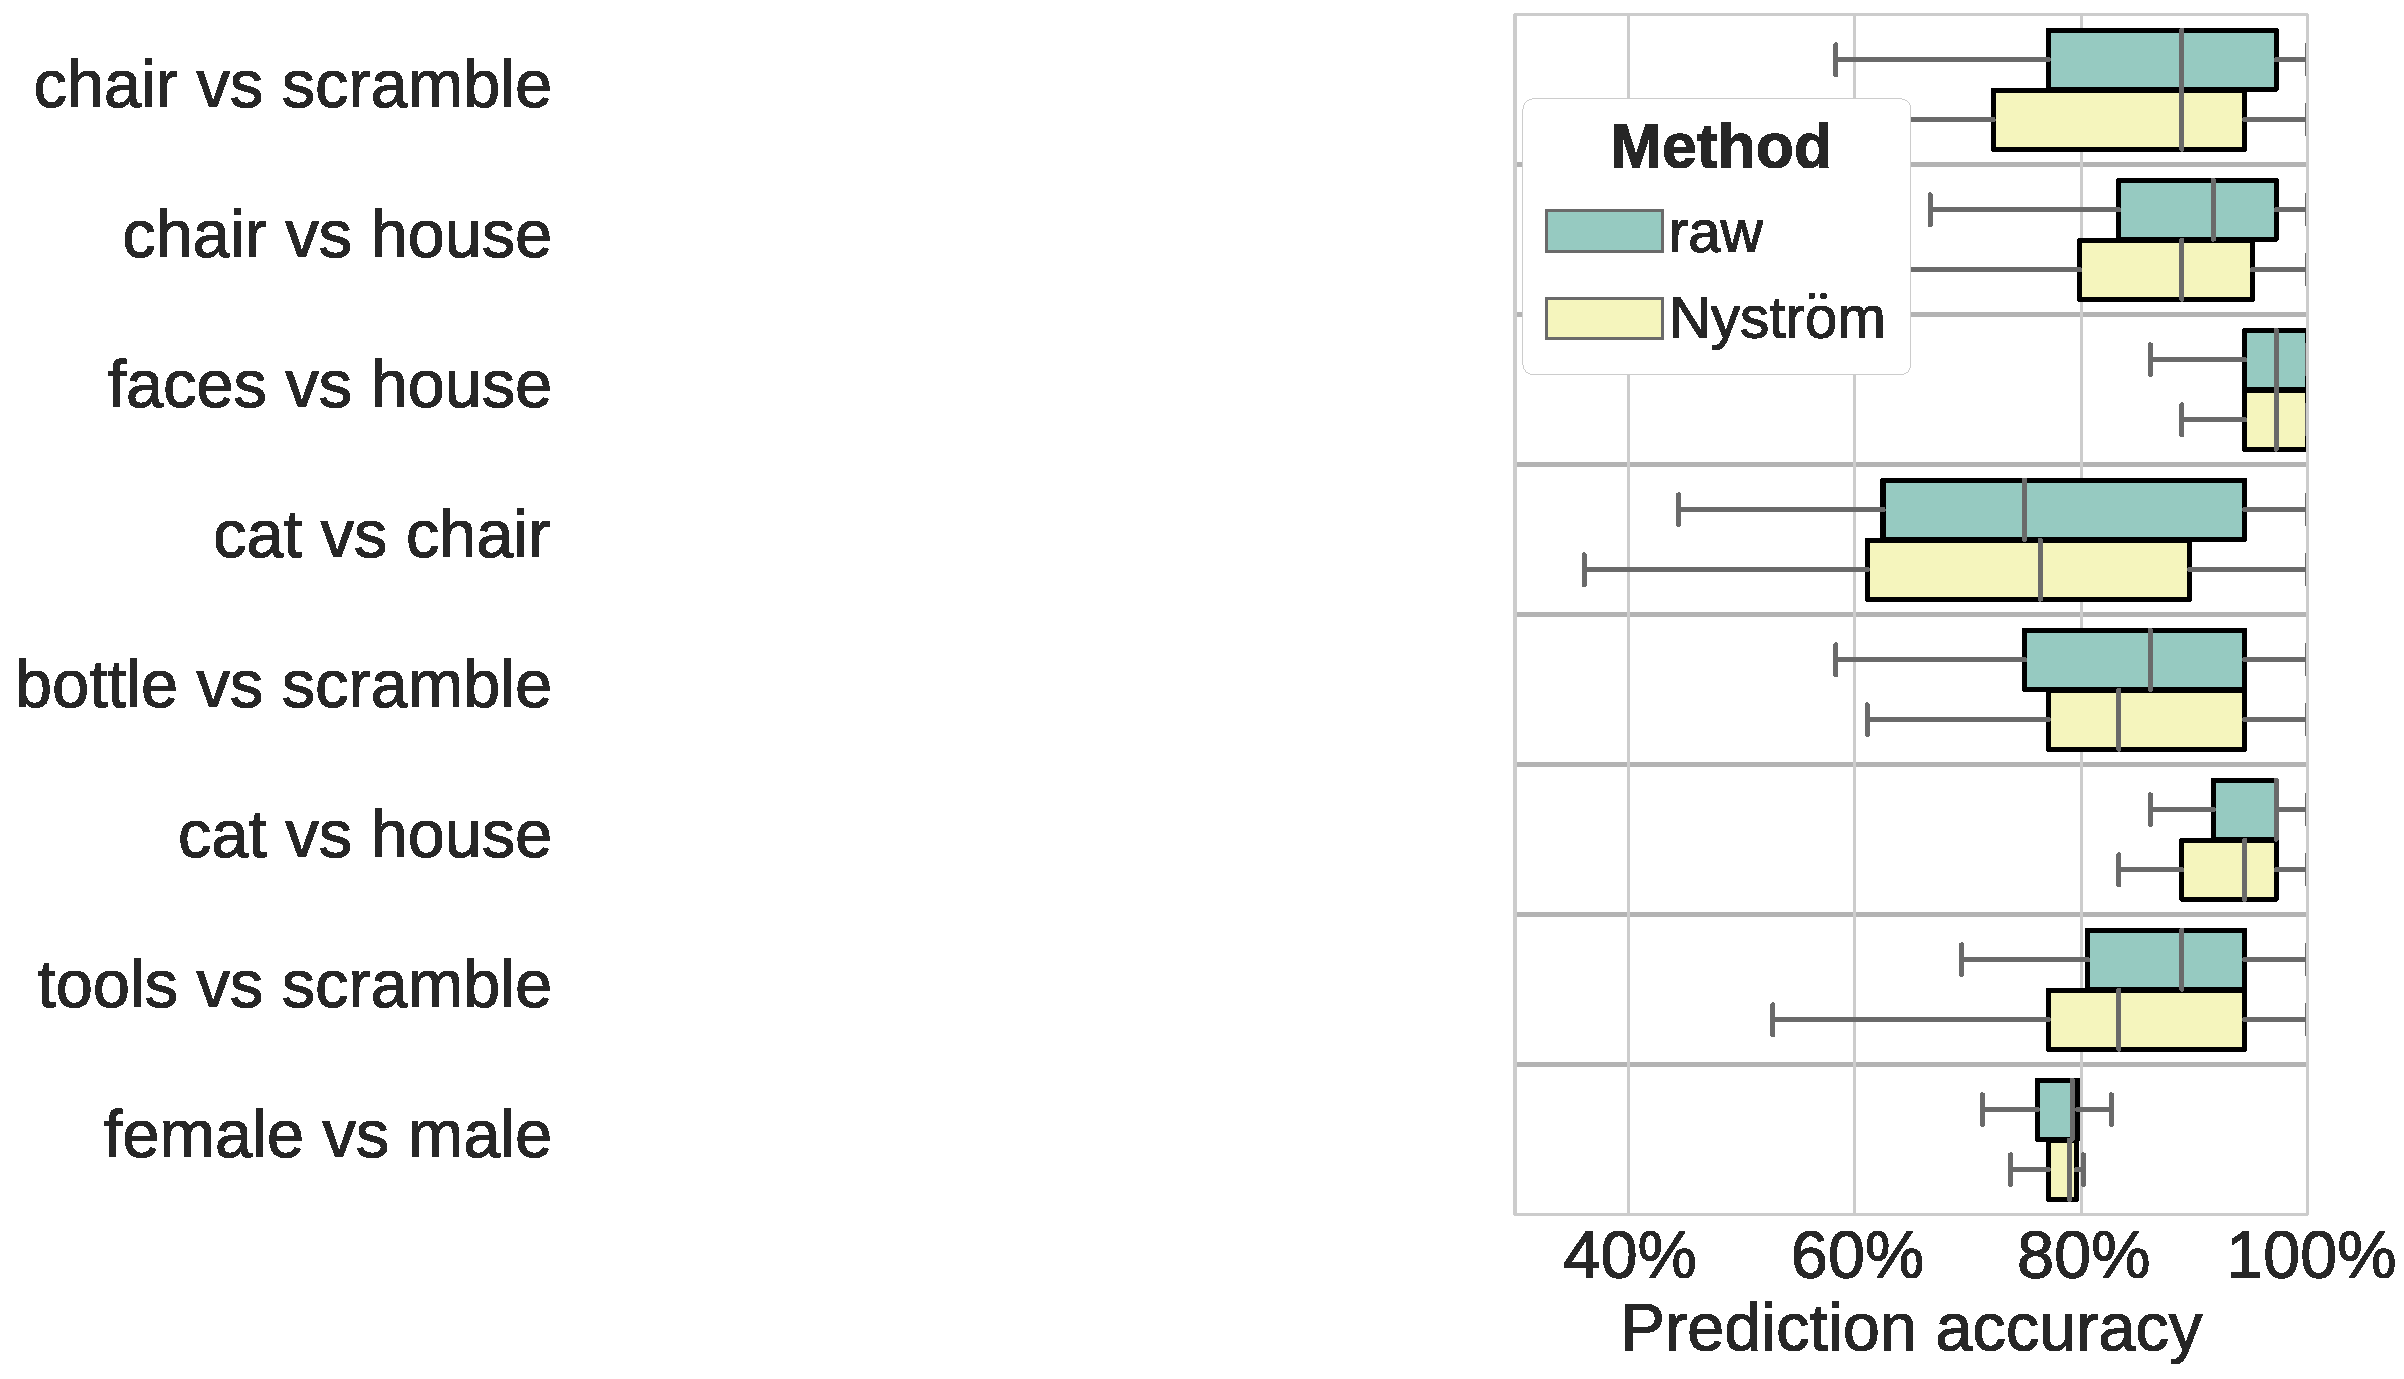
\includegraphics[width=1\linewidth]{figures/correlation_1.pdf}
\caption{\textbf{Consistency of the discriminative weights after dimensionality 
reduction.} Nystr\"om finds consistent maps and it performs as good as raw.}
\end{figure}
\end{frame}


\begin{frame}
\begin{figure}
\centering
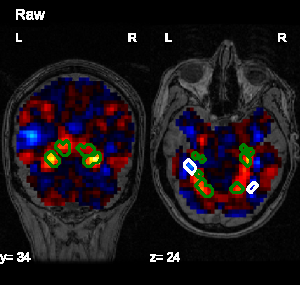
\includegraphics[width=0.43\linewidth]{figures/raw_faces_vs_house_1.pdf}\quad 
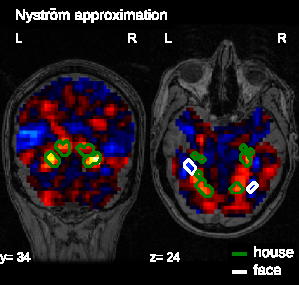
\includegraphics[width=0.43\linewidth]{figures/nystrom_faces_vs_house_1.pdf}
\caption{\textbf{Approximation in the brain space:} Nystr\"om preserves the 
discriminative regions involved in the face and house recognition tasks.}
\end{figure}
\end{frame}


\begin{frame}\frametitle{\textbf{Bringing the reduction to the brain space}}
\begin{figure}
\centering
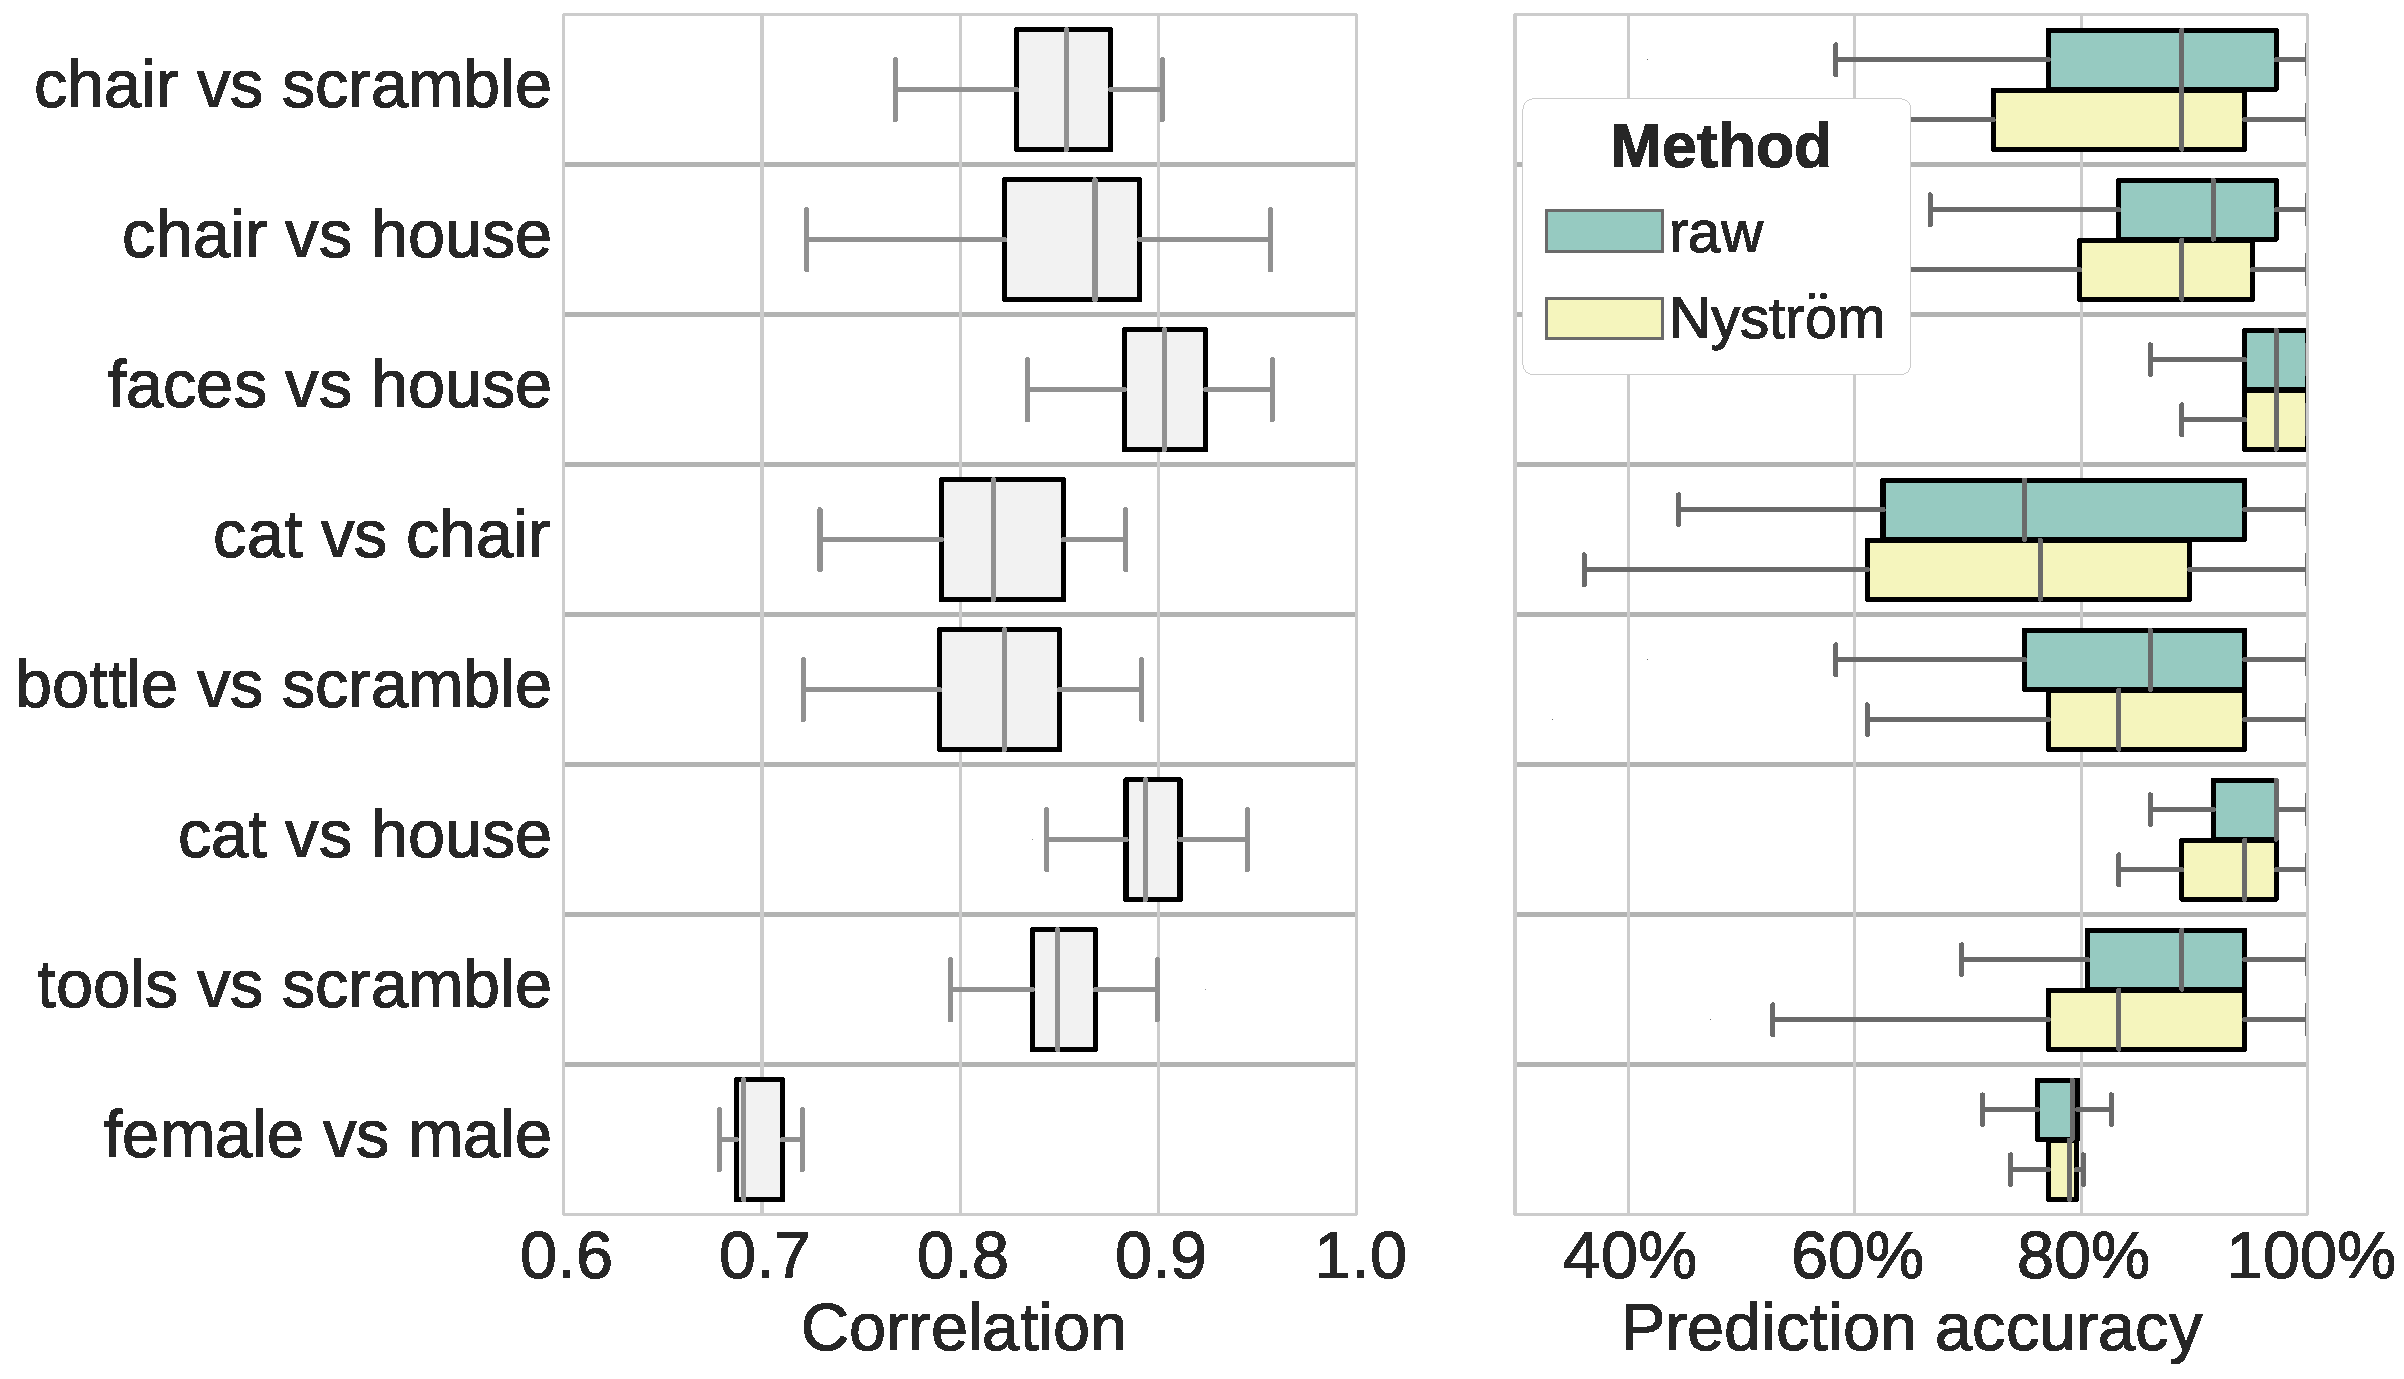
\includegraphics[width=1\linewidth]{figures/correlation.pdf}
\caption{\textbf{Consistency of the discriminative weights after dimensionality 
reduction.} Nystr\"om finds consistent maps and it performs as good as raw.}
\end{figure}
\end{frame}


\begin{frame}\frametitle{\textbf{Conclusion:} Random sampling to go}
\begin{block}{}
\begin{itemize}
\item Nystr\"om and random projections yield \structure{\textbf{impressive 
speed gains}} $> 16$.
\item Nystr\"om finds better solutions than random projections with 
\structure{\textbf{the same time budget}}.
\item For a large-scale dataset (HCP), Nystr\"om \structure{\textbf{speeds up}} 
the 
decoding by a factor of $\approx 280$.
\item Nystr\"om for linear kernels can be \structure{\textbf{brought back}} 
into the brain space.
\item \structure{\textbf{Data-driven methods}} can capture the underlying 
structure of brain images.
\end{itemize}
\end{block}

\begin{figure}

\includegraphics[width=0.3\linewidth]{figures/scikit-learn-logo.png}\hfill

\includegraphics[width=0.3\linewidth]{figures/nilearn-logo.png}
\end{figure}

\end{frame}

\begin{frame}\frametitle{References}
\bibliographystyle{amsalpha}
\bibliography{biblio.bib}
\end{frame}

\end{document}